\documentclass{article}
\usepackage[utf8]{inputenc}

\title{Chem132A: Midterm 1 Solutions}
\author{Moises Romero, Shane Flynn}
\date{October 2017}


\usepackage{graphicx}
\usepackage{amsmath}
\usepackage{braket}
\usepackage[margin=0.7in]{geometry}
\usepackage[version=4]{mhchem}


\newcommand{\be}{\begin{equation}}
\newcommand{\ee}{\end{equation}}
\newcommand{\pd}{\partial}

\begin{document}

\maketitle


\section{Definitions}
\subsection*{Intensive/Extensive}
For each of the following indicate if it is an \textbf{Intensive} or \textbf{Extensive} property.

\bigskip

\begin{tabular}{ l | c }
    Volume & Extensive\\
    Mass & Extensive\\
    Entropy & Extensive\\
    Density & Intensive\\
    Internal Energy & Extensive\\
    Pressure & Intensive\\
    Temperature & Intensive\\
    Gibbs Free energy & Extensive\\
    Helmholtz Free Energy & Extensive\\
    C$_P$ & Extensive\\
\end{tabular}

\subsection*{State functions}
Indicate whether the indicated properties are state functions or not.

\bigskip

\begin{tabular}{ l | c }
    Temperature & Yes\\
    Gibbs Free energy & Yes\\
    Work & No\\
    Heat & No\\
    Entropy & Yes\\
\end{tabular}

\newpage

\section{Phase Diagram}
\begin{figure}[h]
\centering
\caption{Point 1: (P$_1$,V$_1$,T$_1$),\quad Point 2: (P$_2$,V$_2$,T$_1$), \quad Point 3: (P$_1$,V$_2$,T$_3$).}
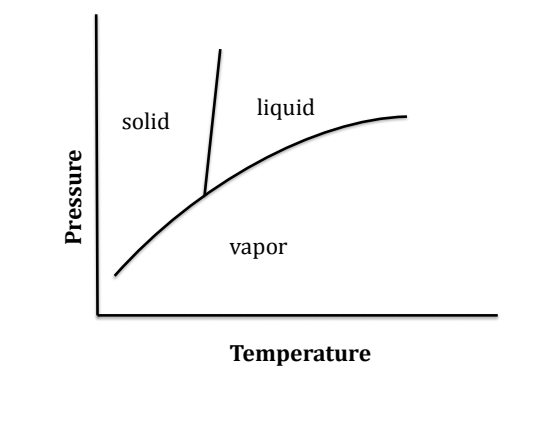
\includegraphics[width=0.5\textwidth]{midterm2.png}
\end{figure}

Consider the phase diagram shown above. 

\bigskip

Is the difference in molar volumes $\left[V_m(\text{liquid}) - V_m(\text{solid})  \right]$ positive or negative? 
State clearly how you arrive at your answer. 
A simple 'positive' or 'negative' without any explanation will receive no credit. 

\bigskip

We are asked about the molar volume, so it may be useful to recall the definition. 
\be
\left(\frac{\pd G}{\pd P}\right)_T = \left(\frac{\pd \mu}{\pd P}\right)_T  = V_m
\ee

Specifically we are interested in the solid to liquid molar volume transition, so we need to focus on the solid to liquid phase line. 

The slope for this transition is positive which suggests the molar volume difference between the liquid and solid state (V$_m$(liquid) - V$_m$(solid)) must be positive. 

\newpage



\section{Free Energy Calculations}

\subsection*{Reversible Work}
Consider a reversible, constant temperature process. 
Starting from the definition of the Helmholtz Free Energy, show that the Helmholtz Free Energy is equal to the reversible work for the process. 

\bigskip

\be
    \begin{split}
    A &= U - TS\\
     d A &= d U - d(TS) \\
        d A_r &= dU_r - T d S_r \\
      d A_r   &= d U_r - T\frac{\delta q_r}{T} \\
       d A_r  &= d U_r - \delta q_r \\
       d A_r  &= \delta q_r + \delta w_r - \delta q_r \\
        d A_r &= \delta w_r
    \end{split}
\ee

\subsection*{Maximum Work for Propane Combustion}
Consider the reaction associated with the combustion of propane: 
\be
\ce{C3H8(g) + O2(g) -> CO2(g) + H2O(l)}
\ee

Assuming propane is an ideal gas and a constant temperature of 298K, compute the maximum work that can be obtained from the combustion of propane: 

Given at 298K: 
\be
\Delta G_{\text{rxn}}^0 = -2108 \frac{\text{kJ}}{\text{mol}} \quad R = 8.314 \frac{\text{J}}{\text{mol-K}}
\ee

\bigskip

Balance the equation!
\be
\ce{C3H8(g) + 5O2(g) -> 3CO2(g) + 4H2O(l)}
\ee

\be
\begin{split}
\Delta A_{\text{rxn}}^0 &= \Delta U_{\text{rxn}}^0-T \Delta S_{\text{rxn}}^0 \\
\Delta A_{\text{rxn}}^0 &= \Delta H_{\text{rxn}}^0 - \Delta (PV) - T\Delta S_{\text{rxn}}^0\\
\Delta A_{\text{rxn}}^0 &= \Delta G_{\text{rxn}}^0 - \Delta (PV)\\
\Delta A_{\text{rxn}}^0 &= \Delta G_{\text{rxn}}^0 - \Delta n_g RT\\
\Delta A_{\text{rxn}}^0 &= (-2108)-(-3)(0.008314)(298) = -2101\frac{\text{kJ}}{\text{mol}} = w_{\text{max}}
\end{split}
\ee

\newpage

\section{First and Second Law}

\subsection{State Functions}

Consider the following diagram for one mole of a gas. 
For this system, all processes are done reversibly and the Internal Energy of the gas is only a function of temperature.


\begin{figure}[h]
\centering
\caption{Point 1: (P$_1$,V$_1$,T$_1$),\quad Point 2: (P$_2$,V$_2$,T$_1$), \quad Point 3: (P$_1$,V$_2$,T$_3$).}
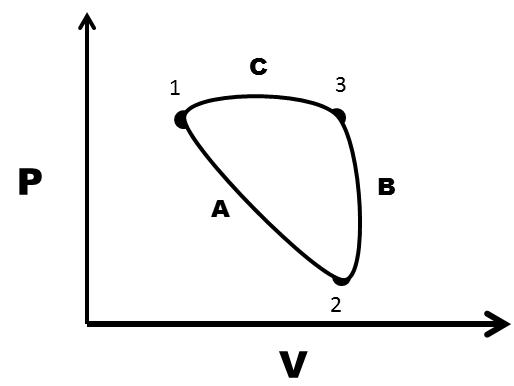
\includegraphics[width=0.5\textwidth]{midterm3.png}
\end{figure}

Only consider PV work for this problem. 
Calculate the change in Internal Energy ($\Delta$U) , the change in Entropy ($\Delta$S), the Heat (q), and the work (w) associated with pathways A,B, and C. 

\bigskip

\subsubsection*{Pathway A} 
Reversible, Isothermal; therefore $\Delta$T=0: 
\be
\Delta U = 0 
\ee
Since U is only a function of temperature. We can then write our first law as : 
\be
q_A=- w_A=\int_{V_1}^{V_2} P_{gas} dV
\ee
With this expression we can determine the Entropy of pathway A as : 
\be
\Delta S_A = \frac{q_{Ar}}{T} = \frac{\int_{V_1}^{V_2} P_{gas} dV}{T}
\ee

\subsubsection*{Pathway B}
This pathway is Isochoric therefore $\Delta$V = 0 so :
\be
w_B = 0 
\ee

The first law is then : 
\be
\Delta U_B = q_B = \int_{T_1}^{T_3} Cv(T) dT
\ee
The Entropy of the system can be expressed as: 
\be
\Delta S_B = \frac{q_B}{T} = \frac{\int_{T_1}^{T_3} Cv(T) dT}{T}
\ee

\subsubsection*{Pathway C}
Pathway C is an Isobaric process so the First Law does not simplify:
\be
\Delta U_C = q_C + w_C 
\ee

The work can be written as : 
\be
w_C = -\int_{V_1}^{V_2} P_{gas} = -P_1\Delta V
\ee
We then use the heat capacity to determine the Internal Energy just as before
\be
\Delta U_C = \Delta U_A + \Delta U_B = \int_{T_1}^{T_3} Cv(T)dT
\ee
Then we rearrange the first law and compute the heat: 
\be
q_C =  \int_{V_1}^{V_2} P_{gas} dV +\int_{T_1}^{T_3} Cv(T)dT
\ee
Since Entropy is a state function it can be expressed as : 
\be
\Delta S _C = \Delta S_A + \Delta S_B =  \frac{\int_{V_1}^{V_2} P_{gas} dV +\int_{T_1}^{T_3} Cv(T) dT}{T}
\ee

\newpage

\section{Enthalpy of Combustion}
Consider the combustion of ethanol under constant pressure conditions (1atm) and at a temperature of 370K. 
The balanced reaction for this combustion is shown below. 
Use the data provided here to calculate the $\Delta$H$_{\text{rxn}}$(370K).

\be
\ce{CH3CH2OH(g) + 3O2(g) <=> 2CO2(g) + 3H2O(l)}
\ee

\subsection*{Formation of Ethanol Gas}
We are only given information about the liquid state of ethanol, we need the enthalpy associated with Ethanol gas. 
This is done by taking the formation enthalpy of the liquid, heating the liquid to the normal boiling point, doing the phase transition to a  gas, and then heating the gas to the final temperature. 
\be
\begin{split}
\Delta H(\text{etoh},370,g) &= \Delta H_f(298,l) + \Delta H(l,298\Rightarrow 351.45) + \Delta H_{vap}(351.45) + \Delta H(g, 351.45 \Rightarrow 370)\\
&= -277.69 + \int_{298}^{351.45} C_P(l)dT + 38.6 + \int_{351.45}^{370} C_P(g) dT \\ 
&= -277.69 + 0.11146(351.45-290) + 38.6 + 0.06544(370-351.45) \\
\Delta H(\text{etoh},370,g) &= -231.919 \frac{\text{kJ}}{\text{mol}}
\end{split}
\ee

\subsection*{Oxygen Gas}


\be
\begin{split}
\Delta H(O_2,g, 370) &= \Delta H_f(298,g) + \int_{298}^{370} C_P(g)dT\\
&= 0 + 0.029355(370-298)\\
\Delta H(O_2,g, 370) &= 2.11356
\end{split}
\ee

\subsection*{Carbon Dioxide Gas}

\be
\begin{split}
\Delta H(CO_2,g, 370) &= \Delta H_f(298,g) + \int_{298}^{370} C_P(g)dT\\
&= -393.51 + 0.03711(370-298)\\
\Delta H(CO_2,g, 370) &= -390.83808
\end{split}
\ee

\subsection*{Water Liquid}
\be
\begin{split}
\Delta H(H_2O,l, 370) &= \Delta H_f(298,l) + \int_{298}^{370} C_P(l)dT\\
&= -285.83 + 0.075291(370-298)\\
\Delta H(H_2O,g, 370) &= -280.409
\end{split}
\ee

\subsection*{Reaction}
Now that we have calculated the heat associated with each component at the final temperature, we simple need to subtract values. 

\be
\begin{split}
\Delta H_{\text{rxn}}(370) &= \sum_i \nu_i \Delta H_i \\
&= 2(\Delta H(CO_2,g, 370)) + 3(\Delta H(H_2O,l, 370)) - 3(\Delta H(O_2,g, 370)) - (\Delta H(\text{etoh},370,g)) \\
&= 2(-390.83808) + 3(-280.409) - 3(2.11356) - (-231.919) \\
\Delta H_{\text{rxn}}(370) &= -1397.325 \frac{\text{kJ}}{\text{mol}}
\end{split}
\ee




\end{document}
